\chapter{Implementation}
In this chapter, we will describe how we implemented the application. We will start explaining the architecture from a high-level perspective with each component being a black-box. Later sections of this chapter will then further describe the internals of every component.

We have implemented our application following the "`single page application (SPA)"' architecture. Some reasons that lead to this decision:
\begin{itemize}	
	\item Due to our personal interest in JavaScript and our intention of improving our knowledge in this language, we wanted a significant part of the development to be done client-side
	\item We imagined the state handling to be easier with a SPA than having to pass around cookies, session data, local storage etc. between every request
	\item A SPA seemed great for building modern looking, intuitive and responsive user interfaces
\end{itemize}

From a high level perspective and following the SPA approach, we have structured our application into 3 main components:

\begin{center}
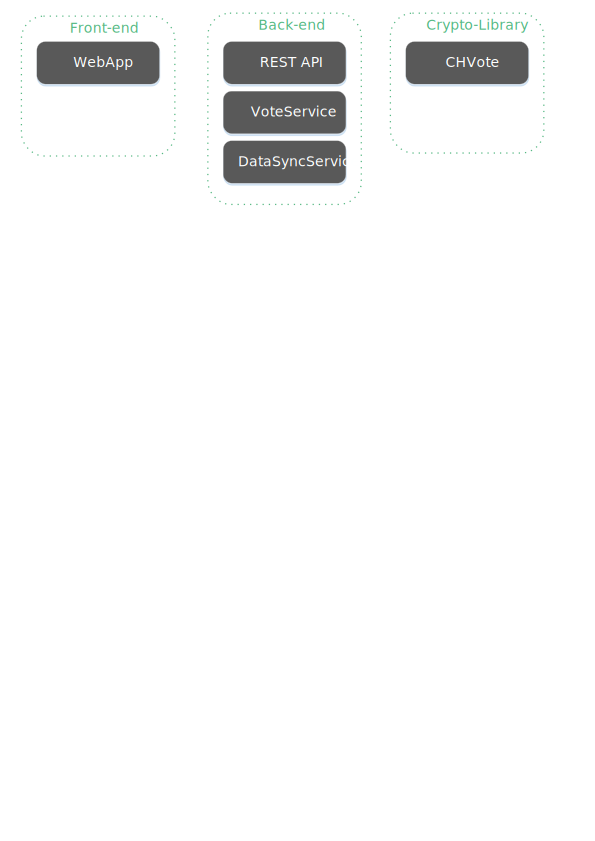
\includegraphics[scale=0.95]{assets/componentdiagram.png}
\captionof{figure}{System components}\label{System components}%
\end{center}

	\item The front-end basically is the JavaScript based web-application where all the functionality of our back-end is consumed and where a typical CHVote election event is visualized.
	\item The \textbf{CHVote crypto-library} is the result of our "`Project 2"' course project which we have finished before our bachelor thesis. This library contains all the algorithms that are specified as pseudocode in the specification document.
	\item The \textbf{back-end} consists of several components that make use of the CHVote crypto-library to build an actual e-voting ecosystem and providing an API to manipulate the data as well as a data sync service to synchronize data from the back-end to the web-clients. All the sub-components of the backend run on a single server.
\end{itemize}

\section{Technology \& Language Decisions}
When we implemented the CHVote crypto-library, we have evaluated and decided to use Python. Since Java has already been used by the team in Geneva, we wanted to use a different language as it was desirable to prove that the CHVote specification can be implemented regardless the programming language. Python seemed like a rather suitable language due to the following reasons:
\begin{itemize}	
	\item python is a mature language with lots of libraries
	\item python's syntax enables programs to be written in a compact and readable style
	\item as the protocol wasn't completely specified at that point and has still been undergoing some changes, we wanted to use a language in which we can adapt changes quickly and easily
	\item native support for large integers (\textit{BigInts}) and bindings for the GMP\footnote{GMP is a free library for arbitrary precision arithmetic, operating on signed integers, rational numbers, and floating-point numbers, see \url{https://gmplib.org/}.} library
	\item supports a lot of platforms
	\item many popular web development frameworks are available
\end{itemize}

Throughout the project not all of the reason above turned out to be true or ideal. The drawbacks that we have experienced during the implementation of this project will be discussed at the end of this document.

Since we used the crypto-library in our back-end, Python was also the obvious language for the back-end. Python offers a wide variety of frameworks for building web-services. Since we planed on building a single-page-application for the client, we chose the lightweight micro-framework flask for building a restful web-service. 

For our \textbf{front-end} (web application) we evaluated several single-page application (SPA) frameworks. VueJS is a new, modern and lightweight SPA framework that in contrast to Angular has a much flatter learning curve but still offered all the functionality that we needed. The VueJS addon Vuex enabled us to establish a data-store pattern in our front-end, which makes it possible to have a copy of the back-end data-store in our web application which is synchronized in real-time through web-sockets.

\textbf{Socket.io} simplifies the usage of web-sockets and offers fallback technologies such as long-polling in case web-socket is not supported by either the browser or the web-server. Both Flask as well as VueJS have plug-ins that support and integrate socket.io.

For persisting the state of an election, we decided to use mongoDB. The reason behind this choice will be described in more details later on.

\section{Architecture}
The core of our application is the VoteService component in our backend which implements the e-voting protocol by utilizing all algorithms of the CHVote crypto-library according to the CHVote specification. The VoteService component internally holds the state of a whole CHVote election and exposes functions to manipulate this state at a granularity required by our web application to implement all use cases. For example: The VoteService contains a list of ballots and exposes functions to cast a new ballot, which will generate a new ballot according to the protocol, by calling the CHVote crypto-library, and adds the ballot to the list.

On top of the VoteService we have implemented a REST service that acts a facade to the VoteService component and makes its functionality available as an API for our web-clients. The REST service also has to initialize the VoteService by loading and persisting it's state from and to the database between each API call.

One of the requirements is that all clients must be informed in real-time about mutations of the election state made by other participants. To achieve this, we have implemented a data sync service which allows to push the state or parts of the state of the VoteService to the web-clients by using the websocket protocol. This service is triggered by the REST service after every API call to push the delta between the old and the new state to the clients.

To establish a proper separation of concerns, the state of the VoteService is always sent to the client via the data sync service. The REST API only returns success or error codes or information that is required in response to some particular API call, and never state objects. On the other hand, the data sync service does never manipulate the state of the VoteService and is solely responsible for sending s to the client.


\begin{center}
\includegraphics[scale=0.62]{assets/architecture.pdf}
\captionof{figure}{Architecture}\label{Architecture}%
\end{center}

From the clients point of view, the web-client contains a copy of the whole VoteService state in a local data-store. This store is initially populated when the web application is initialized with an election. Whenever the state of the VoteService changes, the data sync service pushes the new data to the web application. A local mutation handler within the web application handles those messages and writes the new data into the local data-store.

Since the components that the web-pages of the web application are built of, are directly bound to the local data-store, all mutations are automatically reflected to the user. From those pages, the REST API can again be called to trigger some CHVote specific action on the back end. The resulting state change is again being pushed to all clients while the responsible client that performed the HTTPS request will additionally receive a success code, or an error message in case of an error.

We have decided on this VoteService centric architecture mainly because we wanted to keep all CHVote specific implementation details within a central module and avoid having protocol-specific logic both in the client as well as in the back-end. If the protocol is undergoing any changes or if the demonstrator application should be adapted to another protocol in future, only the VoteService component (and of course its dependencies) will be affected or must be replaced. It also allowed us to implement the CHVote protocol as similar to the specification as possible. Opposed to a real implementation, where all the protocol parties would be running a separate application, it was no problem for our use-cases to have the whole protocol running on one single server and within one process. Because of that, we had access to every actors state and functions from within our VoteService object and could pass data from one actor to another as simple as setting an object property to some value. 
\section{Back-end}
In this section we describe the internals of the back-end services. 
\subsection{VoteService}
The VoteService represents the state of a whole election and holds instances of all the actors that participate in a CHVote election. We have divided the state of a CHVote election into the following classes:

\begin{center}
\includegraphics[scale=0.62]{assets/stateClasses.png}
\captionof{figure}{State classes}\label{State classes}%
\end{center}

\begin{itemize}
	\item \textbf{BulletinBoardState}: Holds all data that is publicly available on the bulletin board (the number of candidates, the tallied result)
	\item \textbf{ElectionAuthorityState}: Holds all data that an election authority knows (e.g. the list of ballots, the secret key of an election authority)
	\item \textbf{VoterState}: Since there is no distinction made between a voter and a voting client in our application, the VoterState contains the data of both the voter (e.g. the voting card) and the data typically known to the voting client (e.g. the points returned by the oblivious transfer)
	\item \textbf{PrintingAuthorityState}: Holds the data known to the printing authority (e.g. the list of all voters private credentials and the voting cards)
	\item \textbf{ElectionAdministratorState}: Holds all data known to the election administrator 
\end{itemize}

Since our application supports that multiple users work on different election events concurrently, the state of an election event cannot be kept in RAM, but needs to be persisted between every single request . For this reason we evaluated different database systems and concepts. We decided not to use a relational database system that requires us to define a database schema as we want our state objects to be the only place where the schema is defined. This "`code-first"' approach makes it easier to apply changes to the protocol in future. 

For our purpose, mongoDB seemed like a good choice. Since we do not need the ability to access and filter our data with arbitrary queries, but only need to be able to save and load a state object of a particular election, we simply store the whole state as a binary string in a mongoDB collection. The only additional attribute that is saved to the database alongside with the serialized state is the electionId which denotes which election a particular state belongs to. An election contains multiple VoterStates and ElectionAuthorityStates. Therefore, these two states additionally require an electionAuthorityId and a voterId.

\begin{center}
\includegraphics[scale=0.62]{assets/db.png}
\captionof{figure}{Example: ElectionAuthority document collection}\label{Example: ElectionAuthority document collection}%
\end{center}

The only common functionality between every state object, is the ability to serialize the object to a JSON string. For this reason we had to write a custom transformer which tells the JSON parser how to serialize data-types such as mpz, bytearrays and custom classes. Luckily, python offers a way to easily serialize any custom object. By calling \mintinline{python}/object.__dict__/ we can convert an object into a dictionary, as long as the transformer is able to serialize all properties of the object.

We described how the state classes are used to divide the data of the VoteService into smaller units. Similarly, the functionality of the VoteService class is separated into classes, one for every actor in the protocol.

\begin{center}
\includegraphics[scale=0.62]{assets/actorClasses.png}
\captionof{figure}{Actor classes}\label{Actor classes}%
\end{center}
The common functionality, namely, a function for loading the corresponding state from the database and one for persisting the state to the database, are contained in an abstract base class.

The distinction between the actors and their states allows us to easily serialize the state of every actor and provide methods for loading and persisting the state to the database.

\begin{center}
\includegraphics[scale=0.62]{assets/votesim.pdf}
\captionof{figure}{State classes}\label{State classes}%
\end{center}
This approach was also necessary because we have implemented the data synchronization between the clients and the back-end using the JSON Patch approach, for which the delta between the original state and the modified state can be automatically determined and operations generated which will patch the state object on the client such that it equals the new, modified state of the back-end. The original state is simply attached as another property to the actor-object. 

\subsection{Data-Sync Service}
One of the big challenges of our application has been the synchronization of the election state from the back-end to the clients local data store. As mentioned earlier, we wanted to achieve real time data synchronization such that every web client observing a particular election, is informed of any change of this elections state. For this purpose we have used web-sockets.

Additionally, we had to keep an eye on the performance of the data transfers since especially the bulletin board and the election authorities grow big in size when they contain a lot of ballots. We observed that the size of the whole state of an election with 6 candidates and 10 voters, of which each has submitted at least one ballot and a confirmation can easily reach 600 kilobytes already. Admittedly, we haven't noticed any performance issues even with rather large elections, however, transferring the whole state of an election after every single mutation didn't seem like a proper solution.

Nevertheless, when a client connects to the data sync service for the first time, it needs to fetch the JSON representation of every state object of the VoteService. For this purpose we have implemented a "`FullSync"' method which will populate the clients local data store with the full state of an election.

\begin{center}
\includegraphics[scale=0.62]{assets/datastores.pdf}
\captionof{figure}{Datastores}\label{Datastores}%
\end{center}
After a client has pupulated his local data store, future manipulations on the backend are synchronized using the so called JSON Patch operations, which only contain the delta between the previous and the current state.

JSON Patch is a structure for describing how a JSON document can be modified / "`patched"'. The procedure is standardized and described in the RFC 6902 of the Internet Engineering Task Force (IETF). There exist JSON Patch implementations for many languages, including Python and JavaScript. We used JSON Patch to realize our incremental data synchronization as follows:

When the VoteService loads the state of its actor objects, it sets the \mintinline{python}/originalState/ property of the actor to a deep copy of the loaded state object. Mutations are always done only to the \mintinline{python}/state/ property. Before calling the \mintinline{python}/persist()/ method on an actor object, we use the Python JSON Patch library to create a set of JSON Patch operations that describes how to patch the \mintinline{python}/originalState/ such that it becomes identical to the manipulated \mintinline{python}/state/ object, by calling 
\mintinline{python}/make_patch(json.loads(self.originalState.toJSON()), json.loads(self.state.toJSON()))/

The result is a JSON array of operations that contains:
\begin{itemize}
	\item The path of the manipulation
	\item The type of operation (replace, add, remove, ...)
	\item The new value (if required)
\end{itemize}

For example, after casting a ballot, we might receive the following JSON patch:

\begin{center}
\includegraphics[scale=0.62]{assets/jsonpatchexample.png}
\captionof{figure}{JSON Patch example}\label{JSON Patch example}%
\end{center}
These JSON patches are pushed to all the clients that need to receive the mutations and are applied to the local datastore which contains the original state. After applying the JSON patch, the data store of all clients contains the same state of an election as the backend.

\begin{center}
\includegraphics[scale=0.62]{assets/datastores_jsonpatch.pdf}
\captionof{figure}{Data-Sync with JSON Patches}\label{Data-Sync with JSON Patches}%
\end{center}
We decided not to use JSON patches when populating the data store for the first time, since generating JSON patches to patch an empty object to the full state of an election could result in thousands of operations that would almost certainly perform worse than sending the whole object over a fast websocket connection.

\subsection{REST API}
The third component of the backend is the REST API. Its responsibility is to serve as an API and to provide all the functionality of the VoteService to the webclients. Every function, such as the \mintinline{python}/castVote()/ has a corresponding endpoint in the REST API service. Since almost every API endpoint looks almost the same, we take a look at one of them:

\begin{minted}[linenos,tabsize=2,breaklines]{python}
@main.route('/castVote', methods=['POST'])
@cross_origin(origin='*')
def castVote():
    data = request.json
    electionId = data["election"]
    selection = data["selection"]
    voterId = data["voterId"]
    votingCode = data["votingCode"]

    if len(selection) == 0:
        return make_error(400, "Empty selection")

    try:        
        sim = VoteSimulator(electionId) # prepare voteSimulator
        
        sim.castVote(voterId, selection, votingCode) # perform action
        
        patches = sim.persist()	# persist modified state and retrieve JSON patches
        
				syncPatches(electionId, SyncType.ROOM, patches)	# send the JSON patches to all clients

    except Exception as ex:
        return make_error(500, str(ex))

    return json.dumps({'result': 'success'})
\end{minted}

The API can be reached by sending a HTTP(S) POST request to our webserver hosting the backend. The URL defines what function will be executed. For example: A POST request to https://<server>:5000/castVote/ would call the above function. The required parameters are added in the POST body.

As a first step, parameters are extracted from the POST request and validated if necessary. As the next step , a VoteSimulator object is instantiated by passing the electionId to the constructor. The VoteSimulator will internally load the states of the corresponding election from the database and instantiate the actor objects such as the election authorities.

Now the VoteSimulator can execute the function which the user intended to call, for example "`CastVote"'. By calling the function \mintinline{python}/persist()/, the new state is written to the database and the JSON Patches of all mutations are determined, returned and can be sent to all clients by calling the Data-Sync service.

The following sequence diagram shows how the vote casting use case is implemented within the backend and how all the components work together.

\begin{center}
\includegraphics[scale=0.62]{assets/votecastingDiagram.pdf}
\captionof{figure}{Vote casting sequence diagram}\label{Vote casting sequence diagram}%
\end{center}

\section{Crypto-library}

\subsection{File structure}
We decided to put every algorithm of the specification in its own file together with related unit tests. The files are structured according to the actors of the protocol, for example:

\begin{itemize}
	\item \textbf{Common}: contains common cryptopgraphic algorithms and the security parameters used by multiple algorithms
	\item \textbf{ElectionAuthority}: contains all the algorithms used by the election authority
	\item \textbf{PrintingAuthority}: contains all the algorithms used by the printing authority
	\item \textbf{VotingClient}: contains all the algorithms used by the voting client
	\item \textbf{ElectionAdministration}: contains all the algorithms used by the election administrator
	\item \textbf{Utils}: contains helper classes and miscellaneous utility functions
\end{itemize}

\subsection{Public parameters}
There exist two types of public parameters:

The \textbf{security relevant parameters}, e.g:

\begin{itemize}
	\item The order of the prime groups: $p$, $\prime{p}$, $\hat{p}$
	\item The length of the voting, confirmation, return and finalization codes
	\item The number of authorities: $s$
\end{itemize}

and \textbf{public election parameters}, e.g.:

\begin{itemize}
	\item The size of the electorate: $N_E$
	\item The number of candidates: $n$
	\item The list of candidate descriptions: $c$
\end{itemize}

The security parameters are typically used within the algorithms and remain unchanged for a longer time period, whereas the public election parameters are only used by the protocol implementations and change with every election.

The object \texttt{SecurityParams} holds all security relevant parameters and is injected as an additional function argument to all algorithms. Several different \texttt{SecurityParams} objects are created initially, which contain all the parameters according to the recommendations in the CHVote specification document ("level 0" for testing purposes and "level 1" through "level 3" for actual use of the protocol). This approach allows us to use different levels of security during development of the algorithms and protocols. For simple unit testing we used "level 0" in order to inject the security parameters recommended for testing puposes. For actual test runs of the project the security parameters from "level 2" were used.

The public election parameters on the other hand are directly passed to the algorithms by the calling party. If an algorithm needs to know certain election parameters (like the size of the electorate $N_E$), these values are typically derived from vectors that they have access to, so they do not require specific knowledge of these parameters.

\subsection{Coding style}
The following source code sample shows a typical implemation of an algorithm (in this exmaple, algorithm 7.18 according to the CHVote specification).

\begin{minted}[linenos,tabsize=2,breaklines]{python}
import unittest
import os, sys
from gmpy2 import mpz
import gmpy2

sys.path.append(os.path.dirname(os.path.dirname(os.path.abspath(__file__))))

from Utils.Utils                    import AssertMpz, AssertList, AssertClass, AssertString
from Crypto.SecurityParams          import SecurityParams, secparams_l0
from Utils.ToInteger                import ToInteger
from VotingClient.GetSelectedPrimes import GetSelectedPrimes
from VotingClient.GenQuery          import GenQuery
from VotingClient.GenBallotProof    import GenBallotProof
from UnitTestParams                 import unittestparams
from Types                          import Ballot
from Utils.StringToInteger          import StringToInteger

def GenBallot(X_bold, s, pk, secparams):
    """
    Algorithm 7.18: Generates a ballot based on the selection s and the voting code X. The
    ballot includes an OT query a and a proof pi. The algorithm also returns the random
    values used to generate the OT query. These random values are required in Alg. 7.27
    to derive the transferred messages from the OT response, which itself is generated by Alg. 7.25.

    Args:
        X_bold (str):                       Voting Code X ∈ A_X^l_X
        s (list of int):                    Selection s = (s_1, ... , s_k), 1 <= s_1 < ... < s_k
        pk (mpz):                           ElGamal key pk ∈ G_p \ {1}
        secparams (SecurityParams):         Collection of public security parameters

    Returns:
        tuple:                              alpha = (r, Ballot) = (r, (x_hat, a, b, pi))
    """

    AssertMpz(pk)
    AssertList(s)
    AssertClass(secparams, SecurityParams)

    x = mpz(StringToInteger(X_bold, secparams.A_X))
    x_hat = gmpy2.powmod(secparams.g_hat, x, secparams.p_hat)

    q_bold = GetSelectedPrimes(s, secparams)                    # q = (q_1, ... , q_k)
    m = mpz(1)

    for i in range(len(q_bold)):
        m = m * q_bold[i]

    if m >= secparams.p:
        return None

    (a_bold, r_bold) = GenQuery(q_bold, pk, secparams)
    a = mpz(1)
    r = mpz(0)

    for i in range(len(a_bold)):
        a = (a * a_bold[i]) % secparams.p
        r = (r + r_bold[i]) % secparams.q

    b = gmpy2.powmod(secparams.g,r, secparams.p)
    pi = GenBallotProof(x,m,r,x_hat,a,b,pk, secparams)
    alpha = Ballot(x_hat,a_bold,b,pi)

    return (alpha, r_bold)

class GenBallotTest(unittest.TestCase):
    def testGenBallot(self):
        selection = [1,4]       # select candidates with indices 1,4
        (ballot, r) = GenBallot(unittestparams.X, selection, unittestparams.pk, secparams_l0)
        print(ballot)
        print(r)

if __name__ == '__main__':
    unittest.main()
\end{minted}

All algorithms contain a short description, which was taken as-is from the specification document, as well as a comment (Google-style documentation string), which can be used to automatically generate code documentation. The algorithm itself is implemented as close to the specification as possible, using the same variable names and (as far as the language supports it) similar control structures:

\begin{itemize}
	\item The suffix \texttt{\_bold} for emphasized (bold) variables, e.g. \texttt{p\_bold} for \textbf{p}
	\item The suffix \texttt{\_hat} for variables with a hat, e.g. \texttt{a\_hat} for $\hat{a}$
	\item The suffix \texttt{\_prime} for variables with a prime, e.g. \texttt{a\_prime} for $a'$
	\item etc.
\end{itemize}

Each file also contains unit test relevant to the specific algorithm (if unit testing was considered useful for the particular algorithm).

The following example shows the similarities between the algorithm pseudo code and the actual implmentation in Python:

\begin{multicols}{2}
\includegraphics[width=0.46\textwidth]{assets/genballot.png}
\columnbreak
\begin{minted}[fontsize=\scriptsize]{python}
x = mpz(StringToInteger(X_bold, secparams.A_X))
x_hat = gmpy2.powmod(secparams.g_hat, x, secparams.p_hat)
q_bold = GetSelectedPrimes(s, secparams)

m = mpz(1)
for i in range(len(q_bold)):
    m = m * q_bold[i]

if m >= secparams.p:
    return None

(a_bold, r_bold) = GenQuery(q_bold, pk, secparams)
a = mpz(1)
r = mpz(0)

for i in range(len(a_bold)):
    a = (a * a_bold[i]) % secparams.p
    r = (r + r_bold[i]) % secparams.q

b = gmpy2.powmod(secparams.g,r, secparams.p)
pi = GenBallotProof(x,m,r,x_hat,a,b,pk, secparams)
alpha = Ballot(x_hat,a_bold,b,pi)

return (alpha, r_bold)
\end{minted}
\end{multicols}

\subsection{Return types}
In most cases, when an algorithm returns more than a scalar datatype, tuples are used. Tuples allow to return multiple values from a function:

\begin{minted}[linenos,tabsize=2,breaklines]{python}
def foo():
   return (1, 2)

def main():
   a, b = foo()
\end{minted}

This way a lot of the source code looked very similar to the pseudo code in the CHVote specification. For more complex data types or return values that are used more often, named tuples were used. The data type "namedtuple" is like a lightweight class and allows access to named properties.

\begin{minted}[linenos,tabsize=2,breaklines]{python}
Ballot = namedtuple("Ballot", "x_hat, a_bold, b, pi")

def main():
   Ballot b = getBallot()
   x_hat = b.x_hat
\end{minted}

By following this approach we can avoid having lots of container classes only used to pass data structures between the algorithms.

\section{Frontend}
Most of the work during our project had to be done for the frontend. Displaying the rather large amount of voting specific data and large numbers required a clean and well structured layout and a modular component design. Luckily, the framework we had choosen, VueJS, did very well in supporting exactly those requirements. We tried to follow the design patterns and best practices proposed by the makers of VueJS wherever possible.

In this section we will explain what concepts of VueJS we used and how we adapted them to our needs.

\subsection{Components}
Components are the basic building blocks of the VueJS framework. The application itself is a component, every page of the application is a component and the pages typically contain lots of components, one for every control like form controls, buttons or custom controls such as the ballot-list etc., which themselves may again consist of multiple components. The concept of components encourages to create reusable modules, provides a way to structure the application and divide it into smaller units and makes the resulting HTML template more expressive and easier to read.

We have created our own VueJS components for every control that we used more than once. For example the ballot list that is shown both on the bulletin board as well as in the election authority view, the labels for displaying truncated large numbers or the cards used as our standard mean for displaying data have all been turned into a custom component. One of the beautiful features of VueJS components is the concept of slots. By defining one or multiple slots within a components template markup, it becomes possible from the parent of a component, to embed content into different locations (slots) within the components HTML template.

We have been using slots to create our card component, which can display information either as the main content of the card, or within an expandable area on the bottom of the card:

\begin{minted}[linenos,tabsize=2,breaklines]{javascript} 
<DataCard title="Foo" :expandable=true>
		Just some text
		<p slot="expandContent">More complex content <BigIntLabel :mpzValue="publicKey"></BigIntLabel>
		</p>
</DataCard>
\end{minted}
The first line "`Just some text"', which gets inserted into the default unnamed slot, could as well be passed as a string parameter to the data card component. However, as things are getting more complicated, one might like to place arbitrary HTML or even another VueJS component inside the expandable content of our datacard. In such cases, component parameters wont work as they only accept primitive data types. Slots on the other hand allow arbitrary content.
\begin{figure}[h!]
\begin{center}
\includegraphics[scale=1.0]{assets/datacardexample.PNG}\\
\caption{Vote casting sequence diagram}
\end{center}
\end{figure}
The following code shows how the data-card component is implemented:

\begin{minted}[linenos,tabsize=2,breaklines]{html} 
<template>
    <v-card class="dataCard">
        <ConfidentialityChip v-if=showConfidentiality"' :type="confidentiality" class="confidentialityChip" />
        <v-card-title primary-title class="dataCardTitle">
            <div><span class="label grey--text">{{title}}
              <v-tooltip top>
                <v-icon v-if="!disableTooltip" color="grey lighten-1" slot="activator">info</v-icon><span>Programmatic tooltip</span>
             </v-tooltip></span>
            </div>
        </v-card-title>
        <v-card-text class="dataCardContent">
                <slot></slot>
        </v-card-text>
        <v-card-actions v-show="expandable">
            <v-btn icon @click.native="showExpander = !showExpander">
                <v-icon>{{ !showExpander ? 'keyboard_arrow_down' : 'keyboard_arrow_up' }}</v-icon>
            </v-btn>
        </v-card-actions>
        <v-slide-y-transition v-show="expandable">
            <v-card-text v-show="showExpander">
                <slot name="expandContent">
                </slot>
            </v-card-text>
        </v-slide-y-transition>
    </v-card>
</template>
<script>
    import { mapState } from 'vuex'

    export default {
      data: function () {
        return {
          showExpander: false
        }
      },
      computed: {
        ...mapState({
          showConfidentiality: state => state.showConfidentiality
        })
      },
      props: {
        title: {
          type: String,
          required: true,
          default: 'Title'
        },
        expandable: {
          type: Boolean,
          required: true,
          default: false
        },
        confidentiality: {
          type: String,
          required: true,
          default: 'public'
        },
        disableTooltip: {
          type: Boolean,
          required: false,
          default: false
        }

      },

      mounted () {
      }
    }
</script>
\end{minted}
The first part within the \mintinline{javascript}/<template>/ tag describes the HTML markup as well as the slots that we have just mentioned.

The \mintinline{javascript}/<script>/ tag contains the actual logic of the component. The \mintinline{javascript}/data/ object contains variable which are defined and valid only locally within the component.  The \mintinline{javascript}/computed/ object maps variables from our central data-store to a local variable which is reactively bound to the data-store. Whenever the value of the given variable changes in the data-store, the computed property is automatically updated in this component. From the template, we can access both local data as well as computed properties. Computed properties can also be used whenever a local variable needs to be formatted, or in some way manipulated for displaying in the components template.

The third source of data are `props`, which are passed as arguments from the parent component. They are typically used to defined options for a component.

Additionally, components may contain \mintinline{javascript}/methods/, typically used for event-handlers like button clicks and event hooks like \mintinline{javascript}/mounted/, \mintinline{javascript}/beforeDestroy/, \mintinline{javascript}/beforeCreated/ to influence the components creation/destruction at different times during the components lifecycle

\subsection{Centralized Data-store \& Flux pattern}
One of the big challenges regarding the architecture of our front-end, was about how and where we would store all the data of an election. Clearly, since we have already divided the elections data into one state for every actor and given that every actor also has it's corresponding view in our front-end, simply storing the data to the respective component has been our first thought. Although a voter mainly needs to access his own data contained in the voters state, some data is to be shared between components, for example the information on the bulletin board.

Since we wanted to avoid having to keep data redundant in multiple components, we have decided to use the Flux design pattern for our front-end. The basic idea of the flux pattern is to have a single, central data source where all the data is stored and which all components have access to. This single data source is called a "`store"' by Flux terminology. VueJS has it's own implementation of the Flux pattern called Vuex. Another important concept is that components can freely access the data in the store, however, they are not allowed to change data, at least not directly. Instead, if a component wants to change data in the store, this has to be done by calling \textbf{mutation functions}. Not allowing direct manipulation of the store makes it much easier to keep track of where mutations came from.

Our web applications data store is divided into multiple modules, one data store module for each corresponding state of the back-end. In reality, all these data stores are part of one single data store, but having multiple modules allows us to structure the mutation and getter functions and help to avoid naming conflicts by having separate namespaces for every module. 

The state of a data-store can be accessed directly from any component by defining a computed property. If the computed properties have to do perform some formatting, aggregation, filtering etc. on the state variables, it is recommended to write getter-functions in the data-store to avoid writing mu
 
\subsection{Internationalization (i18n)}
TODO: I18n

\subsection{Development Environment}
TODO: Webpack, ESlint etc. beschreiben

\section{Challenges}
In this section we describe some of the challenges that we encountered while developing our application. 
\subsection{Websocket subscription concept}
Since our application allows that multiple elections exist at the same time, the question has arised how we could handle that only those clients who are actually observing a particular election receive web-socket messages when an action has been triggered in the respective election.

We have seen similarities between our problem and the one a typical chat has that consists of mutliple chat-rooms in which only those users should be notified of new posts that have actually joined the room. We have adapted this "`chat-room"' concept to our problem by defining a room to be equal to an election.

We can assume that all the pages that actually show data of an election require the elections id to be passed as part of the URL. For example: /BulletinBoard/1 is the route to reach the BulletinBoard view of the election with id 1.

Whenever a route is called that contains the argument `electionId`, we need to make sure that the client has joined this elections room. We therefore set a global variable called \mintinlin{python{/joinedElectionId/ to match the id of the election a user has joined. We created a mixin that can be added to every election page, which makes sure that if the client hasn't yet joined the corresponding election, it emits a "`join"' request to the socket.io server, passing along the electionId:

\begin{minted}[linenos,tabsize=2,breaklines]{javascript}
export default {
  created () {
    if (this.$store.getters.joinedElectionId !== this.$route.params.electionId) { 
		  this.$socket.emit('join', {election: this.$route.params['electionId']}) 
		}
  },
}
\end{minted}
On the server side, we have defined a socket.io listener called "`join"' which will remove the calling client from every room before joining the room of the requested election. There is only exception: The client cannot leave the room that corresponds to the `sid` of the request, since this is basically the channel over which the `join` request is handled.
\begin{minted}[linenos,tabsize=2,breaklines]{python}
@socketio.on('join')
def on_join(data):
    from app.api.syncService import SyncType, fullSync

    electionID = data['election']
    for room in rooms():
        if room != request.sid:
            leave_room(room)
    join_room(electionID)

    from app.api.syncService import emitToClient, SyncType

    fullSync(electionID, SyncType.SENDER_ONLY)

    emitToClient('joinAck', electionID, SyncType.SENDER_ONLY)
\end{minted}

The \mintinline{javascript}/joinAck/ handler in the web application will then set the \mintinline{javascript}/joinedElectionId/ variable to the just joined election id, such that the join will only be called once or until the user chooses a different election.

\section{Automatic Task Processing for election authorities}
In our application, every election authority normally has to manually process all incoming tasks such as ballot checking, confirmation checking, mixing and decrypting. As this can become cumbersome and it might be desirable to perform these tasks manually only for the first election authority, we have implementation an auto-mode in which an election authority automatically performs all tasks. 

There were several different ways how to implement this feature. One possibility would have been building a service which regularly checks for new tasks and processes them. Since every task requires a preceding action (for example: A Ballot-Check-Task requires a voter casting a vote), and since it is reasonable for our use-cases to assume that the authorities perform the tasks sequentially, we have chosen the most simple approach:

When a user casts a ballot and a ballot-check-task is created, we check if the first authority is set to automatic. If yes, the function for checking this ballot is automatically called. This function again checks, if the next election authority is set to automatic and recursively calls itself if that's the case, and so on until one authority has auto-mode disabled.

This means that if the first authority is in manual mode and the other two are set to automatic, they both wait with their execution until the first election authority has manually started executing the task. This strict sequential order is only required for the mixing task, all other tasks could be called in any order. If desired, this behavior could also be implemented with our approach, however, for the moment this is not required.